
\section{Datenanalyse}
Es wurden im Projekt unterschiedliche Daten auf ihre Quantität, Qualität und Verwendbarkeit untersucht. In diesem Schritt betrifft die Datenqualität erstmal die äußerlichen Merkmale, die tatsächliche Ähnlichkeit und der Vergleich von Regendaten folgt in einem späteren Kapitel. 
Für das Projekt werden zum einen die tatsächlichen Niederschlagsdaten in Konstanz zum späteren Vergleich benötigt, zum anderen Radardaten, beides möglichst in ein bis zehnminütlicher Auflösung und möglichst von aktuell bis einige Jahre in die Vergangenheit reichend. 
Wetterradardaten werden von öffentlichen und privaten Anbietern erhoben und sind in unterschiedlichen Qualitäten und unterschiedlicher Datenmenge verfügbar. Der Email-Verkehr mit Meteogroup, einem privaten Wetterdienstleiter zeigte, dass die Daten der Wetterstationen Konstanz Südkurier und Konstanz Dettingen von uns nicht verwendet werden konnten. Die Daten von Windy sind zwar öffentlich zugänglich, jedoch nicht dowloadbar, welches eine Voraussetzung für verwendete Daten ist. Die Daten die Anbieters Kachelmann sind bis ins Jahr 2015 online verfügbar jedoch müssten hier die Nutzungsrechte eindeutig geklärt werden. 
Die umfangreichsten Radardaten werden von der Deutschen Wetterstation zur Verfügung gestellt, daher wurde sich im Team für die Verwendung dieser Daten entschieden. 

\subsection{Verifizierung der Daten}
In den Daten des DWD hat die Konstanzer Wetterstation die ID: 02712. Aus dem Zip-File mit der enthaltenen Textdatei können somit die nun aufgezeigten Daten für die Untersuchung entnommen werden. Zu den wichtigsten Informationen gehören hier das Qualitätsniveau der Daten (zwischen 1 und 16) als QN, das Messdatum im Format YYYYMMDDHHMM, die Niederschlagshöhe und den Niederschlagindikator. Die Aktuellen Daten wurden mit einem Python-Script eingelesen und ein paar kleine Statistiken zum Validieren der Daten vorgenommen. Zum Vergleich wurden hierfür die monatlichen Niederschlagsangaben von Statista.com und Wetterkontor.com genommen, allerdings bezogen die sich auf ganz Deutschland. 
\begin{table}[ht]
\centering
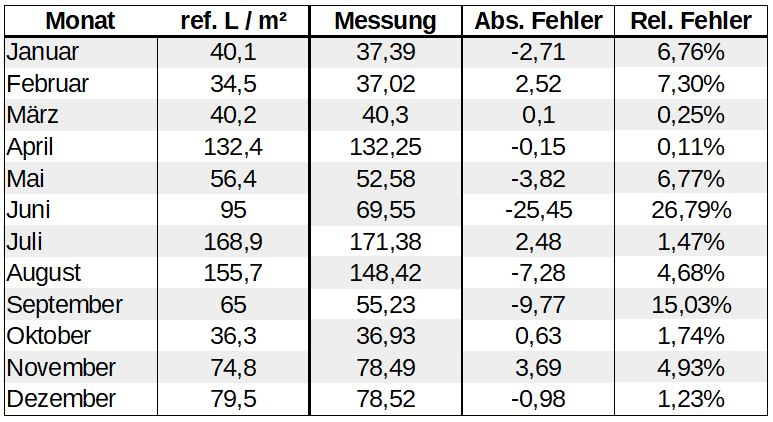
\includegraphics[width=\linewidth]{pics/Auswertung_Thomas}
\caption{(Auswertung des absoluten und relativen Fehlers zwischen den Regendaten verschiedener Quellen)}
\label{tab:Auswertung}
\end{table}
Die Historischen Daten des DWDs sind auch Monatlich als Textdatei gespeichert. Für den Vergleich wurde das Jahr 2018 betrachtet. In den historischen Daten fallen neue Spalten im Header auf, diese sind aber "ungenutzt" bzw. über alle (geprüft auf Jahr 2017) Einträge identisch. Diese sind: QN, RTH_01 und RWH_01. Die Messwerte wurden wie auch zuvor monatsweise zusammenaddiert das Ergebnis des Vergleichs ist in \ref{tab:Auswertung} zu sehen. 
Auffällig ist, dass einige Messwerte sehr gut übereinstimmen. So ist der Niederschlag in den Monaten März und April fast gleich in der referenzierten Messung und der Messung des DWDs. In anderen Monaten wie im Juni ist der relative Fehler mit 26.79 % sehr hoch. Das könnte an gemessenen Extremwerten in den Daten des DWDs liegen, die in der Größenordnung in den Messungen der anderen Anbieter nicht auftauchen.  

\subsection{Korrelation der Radardaten mit den Regenmessungen}

In diesem Schritt sollte geprüft werden, wie hoch die gemessenen Radardaten mit den Niederschlagsdaten korrelieren. Im optimalen Fall sollten alleine auf Grundlage dieser Analyse Rückschlüsse auf die Lage von Konstanz auf dem Radarbildern durch eine besonders hohe Korrelation der Daten möglich sein. Als Monat für die Untersuchung wurde der Juni 2016 gewählt, da es sich um einen sehr Regenreichen Monat gehandelt hat.
Einen wichtigen Anteil an der Korrelationsanalyse hat die Datenaufbereitung in Anspruch genommen. Um einen Vergleich der Niederschlagsdaten mit den Radardaten zu ermöglichen ist es erforderlich, dass die Daten jeweils für dieselben Zeitabstände verfügbar sind. Da die Regenmessungen in minütiger Auflösung vorliegen, wurden sie mit Hilfe zweier Python-Skripte auf eine Datei mit 5-minütiger und eine mit stündlicher Auflösung angepasst. Nun wurde ein Notebook geschrieben, dass die Pixelwerte der Punkte um Konstanz also den Pixelwert 842.406 herum einliest und mit dem Zeitpunkt der Messung und dem tatsächlich gemessenen Niederschlag zu diesem Zeitpunkt in einer Numpy-Matrix speichert. Hier musste eine Einschränkung in Kauf genommen werden, da das einlesen jedes einzelnen Pixels bei 900 x 1100 Pixeln nicht möglich war und daher circa ein Umkreis von 20 Pixeln um Konstanz herum ausgewählt wurde. Bei der ersten Analyse wurde mit 156.377 ein falscher Pixel verwendet, was auf Unklarheiten bei der Achsenbestimmung zurückzuführen war. Die erstellte Numpy-Matrix wurde dann noch auf fehlende Werte untersucht, dieser Anteil hat sich als verschwindend gering herausgestellt, das heißt, dass die Daten bis auf ganz wenige Ausreißer vollständig sind. 
\begin{figure}[ht]
\centering
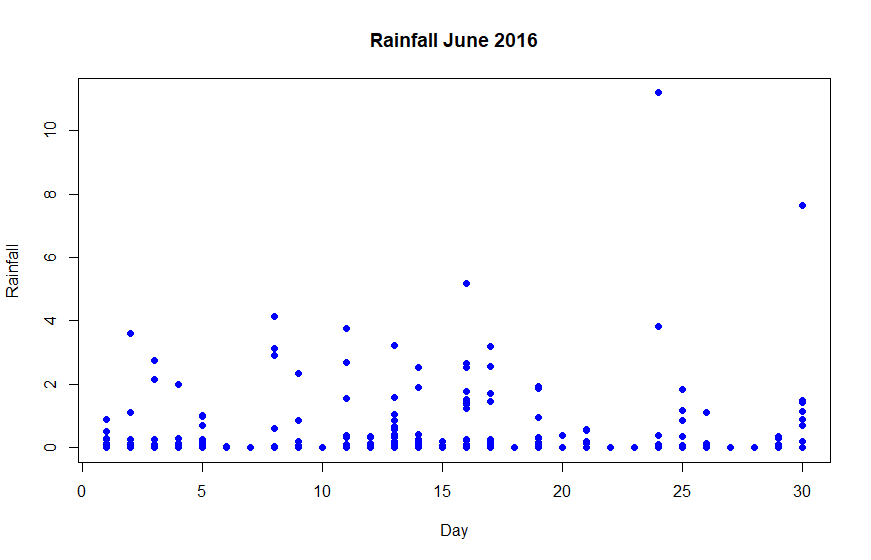
\includegraphics[width=\linewidth]{pics/plot_rainfall_day}
\caption{(Regenfallmengen im Juni 2016 nach Tag)}
\label{fig:Rainfall}
\end{figure}
Für die Analyse der Daten wurde dann ein R-Skript geschrieben. In diesem wurden die Datuminformationen extrahiert, sodass eine Einteilung in Jahr, Monat, Tag, Stunde und Minute der Datensätze möglich wurde. Dann wurden die die Regenmengen der gemessenen Niederschlagswerte je Tag dargestellt. Hier zeigte sich eine recht gleichmäßige Verteilung der Regenwerte mit einigen gut identifizierbaren Ausreißern z.B. am den 24. Juni mit über zehn Liter pro Quadratmeter, siehe \ref(fig:Rainfall}. Bei der Werteverteilung der Pixel aus den Radarbildern fällt auf, dass es sehr viele null-Werte und am zweitmeisten den Wert 80 gibt. Werte, die dazwischen existieren sind „10“, „20“, und „40“.  Bezüglich der Niederschlagsdaten könnte hier auch das eher niedrige Qualitätsniveau der Stufe 3 Einfluss gehabt haben.
Leider konnte zwischen den beiden Datentypen keine Korrelation festgestellt werden. Hierfür kommt eine Reihe von möglichen Gründen in Frage. Da die eigene Betrachtung der Daten, also der händische Abgleich von Zeiten mit Starken Regen in beiden Datengruppen nahelegt, dass die Daten tatsächlich nicht korrelieren kommt in Frage, dass die gemessenen Daten der Wetterstation Konstanz Fehlmessungen beinhalten. 
